\documentclass[a4paper,12pt]{article}

\usepackage[margin=1in,left=1.5in,includefoot]{geometry}
% Graphic
\usepackage{graphicx}
\usepackage{float}

% Hyperlinks
\usepackage{hyperref}

% Header and footer
\usepackage{fancyhdr}
\pagestyle{fancy}
\fancyfoot{}
\fancyhead[LE,RO]{\bfseries\thepage}
\setlength{\headheight}{15pt}

% Quotes character
\usepackage[utf8]{inputenc}

\usepackage{listings}
\lstset{
  basicstyle=\ttfamily,
  columns=fullflexible,
%  frame=single,
  breaklines=true,
  postbreak=\mbox{\textcolor{red}{$\hookrightarrow$}\space},
}

% color links
\usepackage{color}  
\usepackage{hyperref}
\hypersetup{
    colorlinks=true, %set true if you want colored links
    linktoc=all,     %set to all if you want both sections and subsections linked
    linkcolor=black,  %choose some color if you want links to stand out
    urlcolor=blue
}

\begin{document}
\begin{titlepage}
	\begin{center}

\includegraphics[width=0.6\textwidth]{images/Ebi_official_logo}\\[1cm]

{\Large The report}\\[0.5cm]	
	
	\line(1,0){400}\\[0.2in]
	\huge{\bfseries Genome Application}\\
	\line(1,0){400}\\[1.5cm]
	\noindent	
	
%----------------------------------------------------------------------------------------
%	AUTHOR SECTION
%----------------------------------------------------------------------------------------

	
		\begin{center} \large
    	\emph{Authors:}\\
    	Vu Manh \textsc{Tu}\\
		\end{center}

\vfill

% Bottom of the page
{\large \today}
	\end{center}
\end{titlepage}

% Table content
\tableofcontents
\thispagestyle{empty}
\clearpage

\section{The application}
Working web-based application URL: \url{https://genome.glmanhtu.com}\\\\
Genome is a web-based application that archives genomics data and provides a friendly way to interact with those data.\\\\
The application divide into two parts: one is Back-End application, which responsible for things like calculations, business logic, database interactions, performance and another is Front-End application, which is what the user sees, touches and experiences.

\begin{figure}[H]
\centering
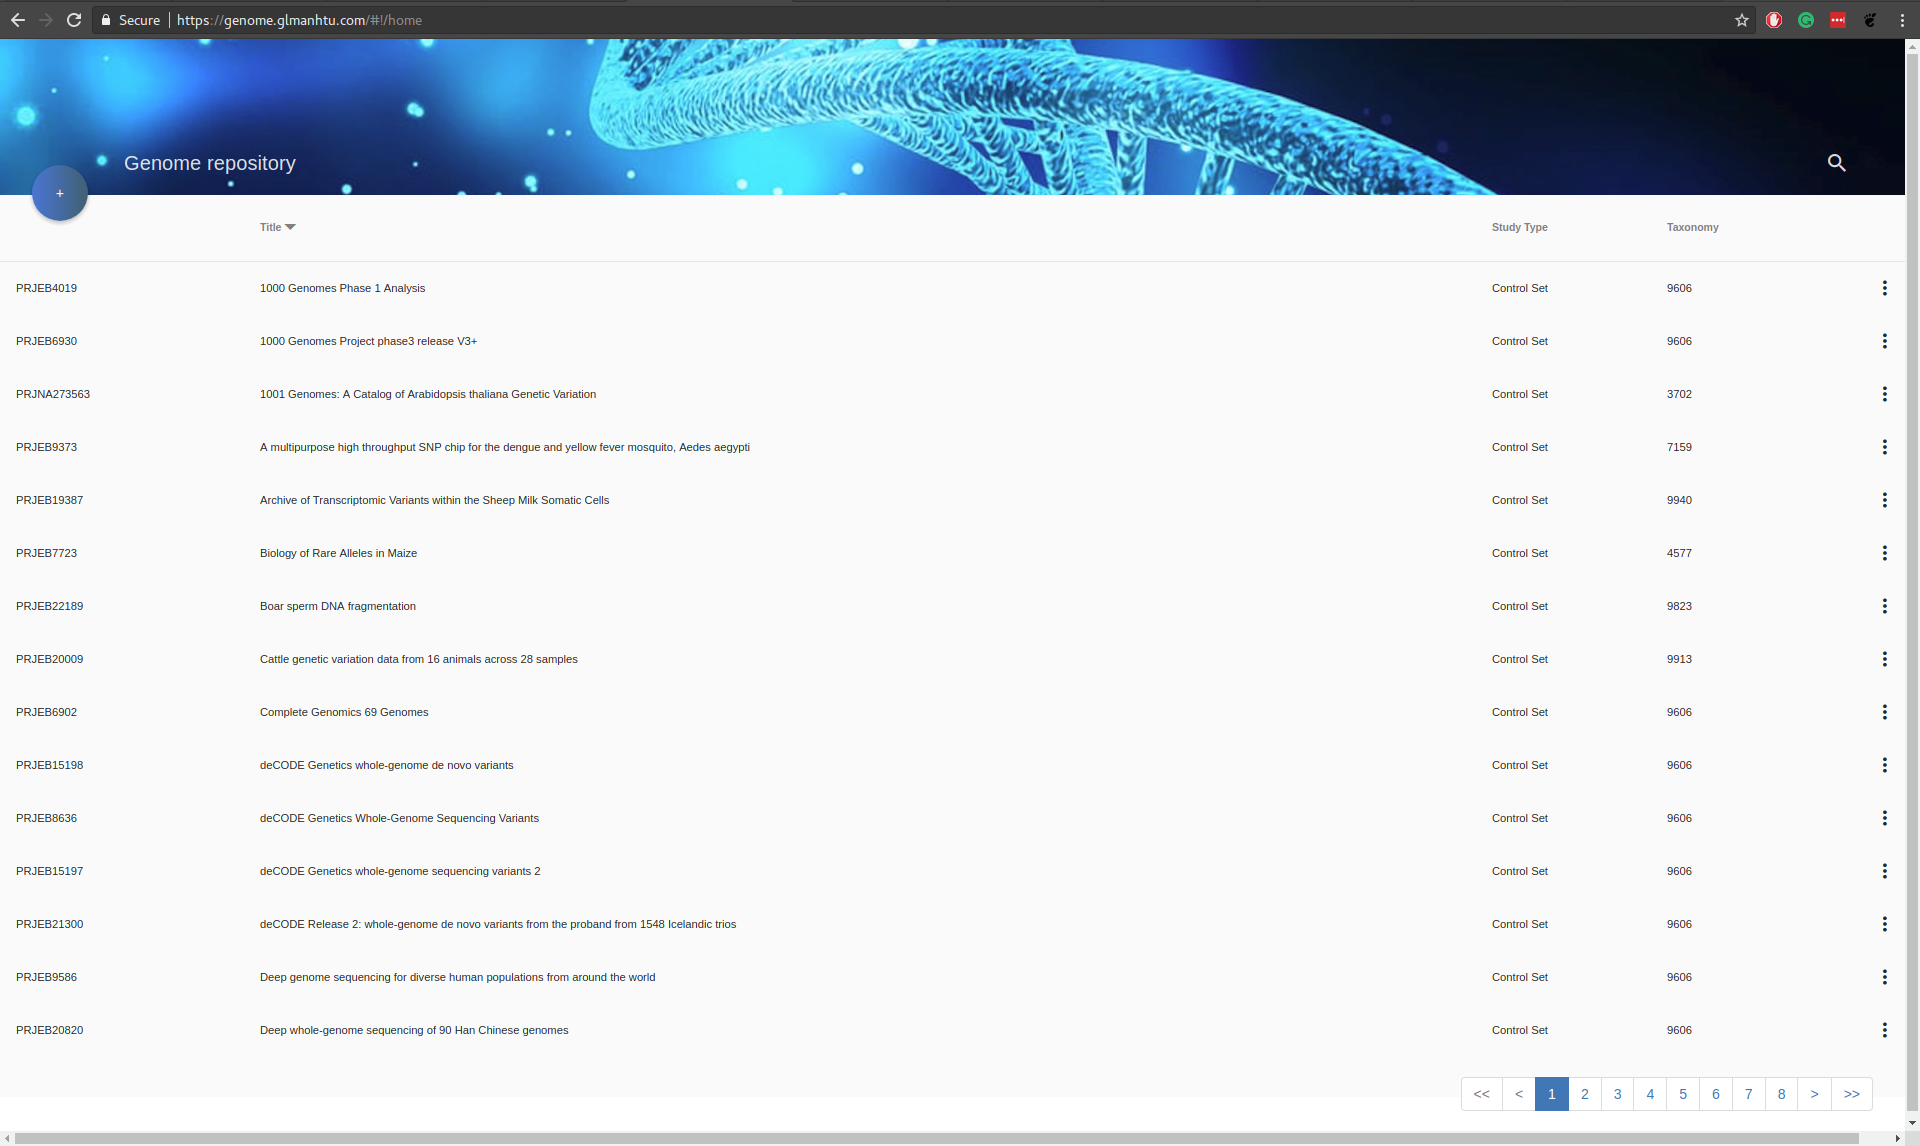
\includegraphics[width=1\textwidth]{images/genome-overview}
\caption{Genome application overview}
\end{figure}

\section{Framework and programming language}
\subsection{The Front-End}
AngularJS is our main framework (\url{www.angularjs.org}) because:
\begin{itemize}
	\item Angularjs require you to split your app into MVC components and then it manages your components for you and also serves as the pipeline that connects them.
	\item Directives achieve this by enabling us to invent our own HTML elements. By putting all our DOM manipulation code into directives, we can separate them out of our MVC app. This allows our MVC app to only concern itself with updating the view with new data.
	\item Filters filter the data before they reach the view and can involve something as simple as formatting decimal places on a number, reversing the order of an array, filtering an array based on a parameter, or implementing pagination. Filters are designed to be standalone functions that are separate from your app, similar to Directives, but are only concerned with data transformations.
	\item All the points up till now mean that you get to write less code. You don’t have to write your own MVC pipeline. The view is defined using HTML, which is more concise. Data models are simpler to write without getters/setters. Data-binding means you don’t have to put data into the view manually. Since directives are separate from app code, they can be written by another team in parallel with minimal integration issues. Filters allow you to manipulate data on the view level without changing your controllers.
	\item Services are exactly what they sound like. They don’t get involved with the MVC of your app, but simply provide an outward API to expose whatever you want it to expose. Most of the time it syncs up to a server to maintain an offline data store and exposes methods to push and pull data to and from a server. Or it can be used to create a resource sharing service that allows multiple controllers to share the same resources.
	\item Data models in Angular are plain old JavaScript objects (POJO) and don’t require extraneous getter and setter functions. You can add and change properties directly on it and loop over objects and arrays at will. Your code will look much cleaner and more intuitive, the way mother nature intended.
\end{itemize}
I also applied some new technical to make the development and
control project easier such as NPM to create a local server, Bower as package control, Gulp as automatic builder tool and SASS to control UI.
\subsection{The Back-End}
I use Java Spring framework and java programming language because:
\begin{itemize}
	\item It's free.
	\item Java Spring is MVC framework base on JavaEE and compatible a huge library of Java can use in this project without problem. In orther hand, Java Spring has supported from very lage Java Comunication. Which Java Spring framework (Spring Boot) was make easier and automatically to config system that help team save a lot of time and avoid errors.
\end{itemize}

\section{Deployment}
I've been implemented both Chef and Docker because of easier for the specific type of users.  With the end-user, they can run direct this application by docker-compose while the developer can deploy their changes and see the result immediately via Chef.
\subsection{Chef}
With Chef Deployment, you can deploy your application, install all dependencies and  configure your clean new virtual private machine (VPS) with a single command. However, it require you to install \& configure Chef workstation. 
\\
\begin{lstlisting}[language=bash]
  $ knife bootstrap <Ip of server> -N '<node name>' -r 'role[<environment>]' --ssh-user <user name on node> --sudo --ssh-identity-file <ssh private credential> --secret-file <location of secret file>
\end{lstlisting}

With `prod` environment, this command will check, install \& configure (if not exist):
\begin{itemize}
	\item \textbf{Oracle Java JDK}
	\item \textbf{Git}: clone or pull changes from git repository
	\item \textbf{Maven}: build project
	\item \textbf{Nginx}: forward port for backend or web-server for frontend
	\item \textbf{NodeJS}: build frontend
\end{itemize}

If your git repository is private, Chef also supports to inject private deploy key and encrypt it via the secret file.
\\\\
Once your VPS bootstrapped, you can easy to re-deploy to get your changes from git repository take effect by one of the following ways:
\\
\\
\indent\textbf{Method 1}: Stay at your workstation and run the following command to re-deploy all your VPS:
\begin{lstlisting}[language=bash]
  $ knife ssh `name:*' `sudo chef-client'
\end{lstlisting}

\textbf{Method 2}: Connect to your VPS and type the following command:
\begin{lstlisting}[language=bash]
  $ sudo chef-client
\end{lstlisting}
\subsection{Docker}
With Docker, you just need to move the terminal console to the source code folder and type the following command:
\begin{lstlisting}[language=bash]
$ docker-compose up
\end{lstlisting}
After that, you can access the application in your browser at \url{http://127.0.0.1}
\end{document}